\documentclass[11pt,a4paper]{article}
\usepackage[utf8]{inputenc}
\usepackage[margin=2.2cm]{geometry}
\usepackage{amsmath,amssymb,amsfonts}
\usepackage{graphicx}
\usepackage{booktabs}
\usepackage{tabularx}
\usepackage{cite}
\usepackage{hyperref}
\usepackage{xcolor}
\usepackage{microtype}
\usepackage{subcaption}

\hypersetup{
    colorlinks=true,
    linkcolor=blue!70!black,
    citecolor=blue!70!black,
    urlcolor=blue!70!black
}

\title{\textbf{Computational Overhead and Scaling in Hybrid Monte Carlo / Molecular Dynamics Simulations of Patchy Colloidal Clusters: Data Transfer Channels, Task Invocation Paradigms, and Tabular Interactions}}

\author{
    \textbf{Eva Gonz\'{a}lez Noya}, \textbf{Antonio D\'{i}az-Pozuelo}, and \textbf{Enrique Lomba}\\[0.5em]
    \textit{Instituto de Qu\'{i}mica F\'{i}sica Blas Cabrera (IQF-CSIC)}\\
    \textit{Serrano 119, 28006 Madrid, Spain}\\[0.3em]
    \small Emails: \texttt{\{eva.noya, adiaz, e.lomba\}@iqf.csic.es}
}

\date{\today}

\begin{document}

\maketitle

\begin{abstract}
Hybrid Monte Carlo (HMC) methods combine canonical Monte Carlo sampling with short microcanonical molecular dynamics (MD) trajectories to bypass kinetic traps in complex condensed-matter systems. Coupling massively parallel GPU-accelerated cellular checkerboard Monte Carlo algorithms with mature external MD engines (such as LAMMPS) presents substantial multi-layered computational overheads: host--device memory synchronization, rigid-body geometric mappings, disk-based versus in-memory coordinate communications, simulation task re-initialization (``forking''), and force-field evaluation dynamics. In this work, we present a rigorous, microsecond-resolution profiling analysis of the HMC interface in \texttt{MC\_Checkerboard} for a cluster-forming system of $N = 7{,}695$ tetrahedral patchy colloidal particles ($38{,}475$ explicit interaction sites) interacting via the Palaia site--site patchy (SSP) model on NVIDIA RTX PRO 4500 (Blackwell architecture). We quantitatively analyze three fundamental architectural aspects: (1) \textbf{Data Transfer Channels}: Disk-based ASCII file formatting and parsing consumes $122.88$~ms per trial, whereas direct in-memory API transfers via \texttt{scatter\_atoms} and \texttt{gather\_atoms} require only $0.43$~ms, yielding a \textbf{$287\times$ acceleration} in coordinate exchange; (2) \textbf{Task Invocation and Forking Paradigms}: In-process library re-initialization with environment reset (\texttt{clear}) incurs a persistent $351.5$~ms setup penalty per trial, whereas maintaining a persistent in-memory simulation topology eliminates this overhead entirely; and (3) \textbf{Potential Representations}: GPU-accelerated linear tabular potentials (\texttt{pair\_style table linear}) with GPU-resident neighbor lists deliver up to a \textbf{$6.66\times$ speedup} in pure MD trajectory propagation compared to continuous analytic overlays (\texttt{hybrid/overlay lj/cut cosine/squared}). Finally, we delineate the crossover trajectory length $N_{\mathrm{md}}^*$ above which physical MD integration dominates over coupling overhead ($N_{\mathrm{md}}^* \approx 20$ for tabular potentials and $N_{\mathrm{md}}^* \approx 4$ for analytic potentials). These findings provide concrete architectural principles for high-throughput hybrid simulation engines intended for modern heterogeneous HPC platforms.
\end{abstract}

\section{Introduction}

Colloidal suspensions featuring directional, valence-limited interactions (``patchy colloids'') exhibit rich equilibrium phase diagrams, self-assembling into open networks, porous gels, and discrete finite-size clusters\cite{sciortino2007patchy,palaia2022patchy,bianchi2006phase}. While Monte Carlo (MC) simulations equipped with localized single-particle displacements and rotations are canonical tools for exploring phase space, dense and strongly associating patchy fluids frequently encounter severe kinetic bottlenecks. In cluster-forming regimes, particles are bound by deep anisotropic potential wells; single-particle trial moves that attempt to dislodge or re-orient a core particle suffer near-zero acceptance rates, while isolated gas-phase monomers explore vast empty interstitial volumes without easily locating cluster interfaces\cite{rovigatti2018simulate,whitelam2007avoiding}.

To circumvent these kinetic bottlenecks, Hybrid Monte Carlo (HMC)\cite{duane1987hybrid,mehlig1992hybrid,forrest1990hybrid} provides an appealing strategy. In HMC, localized stochastic MC cycles are periodically interleaved with short microcanonical ($NVE$) Molecular Dynamics (MD) trajectories of duration $\tau = N_{\mathrm{md}} \Delta t$. Starting from configuration $\mathbf{q}_0$, initial particle momenta $\mathbf{p}_0$ are sampled from the Maxwell--Boltzmann distribution at temperature $T$. The system is integrated deterministically along Hamiltonian trajectories generated by the physical equations of motion:
\begin{equation}
\dot{\mathbf{q}} = \mathbf{M}^{-1}\mathbf{p}, \quad \dot{\mathbf{p}} = -\nabla_{\mathbf{q}} U(\mathbf{q})
\end{equation}
Because symplectic, time-reversible integrators (such as the Velocity Verlet algorithm or symplectic rigid-body integrators\cite{miller2002symplectic}) conserve the total Hamiltonian $H(\mathbf{q}, \mathbf{p}) = U(\mathbf{q}) + K(\mathbf{p})$ up to discretization error $\mathcal{O}(\Delta t^2)$, the trial configuration $(\mathbf{q}_\tau, \mathbf{p}_\tau)$ is accepted or rejected according to the generalized Metropolis criterion:
\begin{equation}
P_{\mathrm{acc}} = \min\left(1, \, \exp\left(-\beta [H(\mathbf{q}_\tau, \mathbf{p}_\tau) - H(\mathbf{q}_0, \mathbf{p}_0)]\right)\right)
\end{equation}
Since all particles undergo collective, momentum-driven displacements along physical force gradients, HMC facilitates collective conformational rearrangements, yielding high acceptance rates even for large-scale moves that would be virtually impossible through random single-particle proposals\cite{neal2011mcmc,forrest1990hybrid}.

Recently, \texttt{MC\_Checkerboard}\cite{gonzalez2026checkerboard} was developed to leverage the massive parallelism of modern GPUs through a 3D checkerboard spatial domain decomposition, achieving sub-second sweep times for tens of thousands of particles. To incorporate HMC, \texttt{MC\_Checkerboard} interfaces directly with the LAMMPS molecular dynamics engine\cite{thompson2022lammps} via the Fortran \texttt{liblammps} API.

However, coupling a high-performance GPU-native Monte Carlo code with a general-purpose MD engine introduces critical performance questions:
\begin{enumerate}
    \item \textbf{Data Transfer Overhead}: How much time is spent transferring coordinates back and forth between GPU checkerboard memory buffers, host memory representations, and LAMMPS internal data structures? Specifically, what is the penalty of file-based communication (dumping formatted ASCII data to disk and reading it via \texttt{read\_data}) versus direct in-memory pointer transfers (\texttt{scatter\_atoms} and \texttt{gather\_atoms})?
    \item \textbf{Task Invocation and Forking Overhead}: What is the relative cost of spawning an external MD process (OS process forking via \texttt{mpirun} / \texttt{system}), resetting an in-process library instance via \texttt{clear}, versus operating with a persistent in-memory simulation state?
    \item \textbf{Potential Representations}: How does evaluating forces via continuous analytic formulas compare against GPU-resident tabulated potentials in terms of initial setup latency, memory footprint, and pure MD propagation throughput?
    \item \textbf{Crossover Scaling}: At what trajectory length $N_{\mathrm{md}}^*$ does the time spent in physical MD integration begin to dominate over the coupling and communication overhead?
\end{enumerate}

In this paper, we present a rigorous, quantitative benchmarking investigation addressing each of these questions. All tests are conducted on an NVIDIA RTX PRO 4500 GPU (Blackwell architecture) for a challenging cluster-forming colloidal fluid of $N = 7{,}695$ particles with tetrahedral patchy interactions ($38{,}475$ explicit interaction sites).

---

\section{System Specifications and Potential Formulations}

\subsection{Site--Site Patchy (SSP) Colloidal Model}

We consider the site--site patchy (SSP) colloidal model introduced by Palaia et al.\cite{palaia2022patchy}. Each colloidal particle $i \in \{1, \dots, N\}$ consists of a central spherical core of diameter $\sigma$ located at position $\mathbf{R}_i$, decorated with $n_p = 4$ attractive interaction sites (``patches'') situated on the core surface at radial distance $r_p = \delta_p \sigma$ ($\delta_p = 0.5$). The four patches are arranged in an ideal tetrahedral geometry:
\begin{equation}
\hat{\mathbf{p}}_1 = \frac{1}{\sqrt{3}}(1, 1, 1), \quad
\hat{\mathbf{p}}_2 = \frac{1}{\sqrt{3}}(1, -1, -1), \quad
\hat{\mathbf{p}}_3 = \frac{1}{\sqrt{3}}(-1, 1, -1), \quad
\hat{\mathbf{p}}_4 = \frac{1}{\sqrt{3}}(-1, -1, 1)
\end{equation}
The orientation of particle $i$ in space is parameterized by a unit quaternion $\mathbf{q}_i = (q_{0,i}, q_{1,i}, q_{2,i}, q_{3,i}) \in \mathbb{S}^3$, which corresponds to the standard $3 \times 3$ orthogonal rotation matrix $\mathbf{R}_{\mathrm{rot}}(\mathbf{q}_i)$:
\begin{equation}
\mathbf{R}_{\mathrm{rot}} = \begin{pmatrix}
q_0^2 + q_1^2 - q_2^2 - q_3^2 & 2(q_1 q_2 - q_0 q_3) & 2(q_1 q_3 + q_0 q_2) \\
2(q_1 q_2 + q_0 q_3) & q_0^2 - q_1^2 + q_2^2 - q_3^2 & 2(q_2 q_3 - q_0 q_1) \\
2(q_1 q_3 - q_0 q_2) & 2(q_2 q_3 + q_0 q_1) & q_0^2 - q_1^2 - q_2^2 + q_3^2
\end{pmatrix}
\end{equation}
The explicit spatial position of patch $k \in \{1, \dots, n_p\}$ on particle $i$ is:
\begin{equation}
\mathbf{r}_{i, k} = \mathbf{R}_i + r_p \, \mathbf{R}_{\mathrm{rot}}(\mathbf{q}_i) \, \hat{\mathbf{p}}_k
\end{equation}
The system comprises $N = 7{,}695$ particles enclosed in a cubic box of side length $L = 39.8263\sigma$, corresponding to a reduced number density $\rho = N/L^3 = 0.1218$. The fluid is a binary mixture containing $N_1 = 1{,}895$ particles of species 1 and $N_2 = 5{,}800$ particles of species 2. In LAMMPS, each rigid colloid is mapped onto 1 core atom and 4 patch satellite atoms, resulting in $N_{\mathrm{sites}} = 5 \times 7{,}695 = 38{,}475$ total interaction sites.

\subsection{Potential Formulations: Analytic vs. Tabulated}

Interactions between colloidal bodies consist of two isotropic contributions:
\begin{enumerate}
    \item \textbf{Core--Core Repulsion and Dispersion Tail}:
    The interaction between the central cores of particles $i$ and $j$ at distance $r_{ij} = \|\mathbf{R}_i - \mathbf{R}_j\|$ is given by a Weeks--Chandler--Andersen (WCA) repulsive core plus an attractive cosine-squared tail:
    \begin{equation}
    u_{\mathrm{core}}(r_{ij}) = \begin{cases}
    4\epsilon \left[\left(\frac{\sigma}{r_{ij}}\right)^{12} - \left(\frac{\sigma}{r_{ij}}\right)^6\right] + \epsilon, & r_{ij} \le 2^{1/6}\sigma \\
    -\epsilon_t \cos^2\left(\frac{\pi (r_{ij} - 2^{1/6}\sigma)}{2(R_c - 2^{1/6}\sigma)}\right), & 2^{1/6}\sigma < r_{ij} \le R_c \\
    0, & r_{ij} > R_c
    \end{cases}
    \end{equation}
    with $\epsilon_t = 0.2\epsilon$ and cutoff radius $R_c = 2.0 \times 2^{1/6}\sigma \approx 2.2449\sigma$.
    \item \textbf{Patch--Patch Anisotropic Attraction}:
    Interaction between patch $k$ on particle $i$ and patch $l$ on particle $j$ at distance $d_{kl} = \|\mathbf{r}_{i,k} - \mathbf{r}_{j,l}\|$ is mediated by an attractive cosine-squared well:
    \begin{equation}
    u_{\mathrm{patch}}(d_{kl}) = \begin{cases}
    -V_{kl} \cos^2\left(\frac{\pi d_{kl}}{2 R_{cp}}\right), & d_{kl} \le R_{cp} \\
    0, & d_{kl} > R_{cp}
    \end{cases}
    \end{equation}
    with interaction strength $V_{kl} = 1.0\epsilon$ and patch cutoff $R_{cp} = 0.3 \times 2^{1/6}\sigma \approx 0.3367\sigma$.
\end{enumerate}

In our benchmarks, we examine two implementations of this potential in LAMMPS:
\begin{itemize}
    \item \textbf{Analytic Mode (\texttt{table\_lammps = .false.})}: Utilizes LAMMPS's \texttt{pair\_style hybrid/overlay lj/cut 20.0 cosine/squared 20.0}. Because the \texttt{cosine/squared} potential in the \texttt{EXTRA-PAIR} package does not support the GPU package neighbor lists, neighbor list builds are performed on the host CPU (\texttt{-pk gpu 1 neigh no -sf gpu}), and pair forces are evaluated analytically.
    \item \textbf{Tabulated Mode (\texttt{table\_lammps = .true.})}: Tabulates all 10 pairwise interactions ($2 \times 2$ central and patch combinations) into linear grids of $M = 100{,}000$ points (\texttt{pair\_style table linear 100000}). This enables full GPU neighbor list acceleration (\texttt{-pk gpu 1 neigh yes -sf gpu}) with hardware-interpolated table lookups executed directly within the GPU streaming multiprocessors.
\end{itemize}

---

\section{Data Transfer and Conversion Layer Overhead}

\subsection{Architecture of the Data Pipeline}

Every HMC cycle requires translating the state of the simulation from the GPU checkerboard cellular representation into LAMMPS, and subsequently re-injecting the evolved state back into the GPU cellular grid. This pipeline comprises four sequential transformation and transport steps (illustrated schematically):
\begin{equation}
\underbrace{\text{GPU Cellular Grid}}_{\text{\texttt{Sphere\_Cell\_dev}}} 
\xrightarrow[\text{De-aggregation}]{\mathrm{T1}}
\underbrace{(\mathbf{R}_i, \mathbf{q}_i)}_{\text{Host Linear Arrays}}
\xrightarrow[\text{Patch Generation}]{\mathrm{T2}}
\underbrace{\{\mathbf{r}_{i,k}\}_{k=0}^{4}}_{\text{5N Explicit Sites}}
\xrightarrow[\text{Transport}]{\mathrm{T3, T4}}
\underbrace{\text{LAMMPS Atom State}}_{\text{Internal C++ Pointers}}
\end{equation}
Upon completion of the MD trajectory:
\begin{equation}
\underbrace{\text{LAMMPS Atom State}}_{\text{Internal C++ Pointers}}
\xrightarrow[\text{Retrieval}]{\mathrm{T6}}
\underbrace{\{\mathbf{r}'_{i,k}\}_{k=0}^{4}}_{\text{5N Coordinates}}
\xrightarrow[\text{Triad Projection}]{\mathrm{T7}}
\underbrace{(\mathbf{R}'_i, \mathbf{q}'_i)}_{\text{Host Linear Arrays}}
\xrightarrow[\text{Re-binning}]{\mathrm{T8}}
\underbrace{\text{GPU Cellular Grid}}_{\text{\texttt{Sphere\_Cell\_dev}}}
\end{equation}

\begin{table}[t]
\centering
\small
\caption{\textbf{Data Transfer and Geometric Conversion Layer Breakdown} for $N = 7{,}695$ colloids ($38{,}475$ explicit interaction sites). Timings represent the arithmetic mean across 5 independent trials on NVIDIA RTX PRO 4500 and host AMD EPYC CPU.}
\label{tab:transfer_breakdown}
\setlength{\tabcolsep}{4.5pt}
\begin{tabularx}{\textwidth}{l>{\raggedright\arraybackslash}Xcc>{\raggedright\arraybackslash}p{3.2cm}}
\toprule
\textbf{Phase} & \textbf{Description} & \textbf{Latency (ms)} & \textbf{Fraction} & \textbf{Transfer Mechanism} \\
\midrule
\texttt{T1} & GPU Checkerboard $\to$ Host Linear (\texttt{Convert\_CB\_RU}) & $0.102$ & $0.08\%$ & GPU $\to$ Host Memory \\
\texttt{T2} & Rigid Body $(\mathbf{R}, \mathbf{q}) \to 5N$ Sites (Patch Gen) & $0.190$ & $0.15\%$ & Geometric Mapping \\
\texttt{T3} & ASCII Serialization to Disk (\texttt{lammps\_hmc.data}) & $47.865$ & $37.66\%$ & Host $\to$ Disk File I/O \\
\texttt{T4} & LAMMPS Text Parsing from Disk (\texttt{read\_data}) & $75.010$ & $59.02\%$ & Disk $\to$ LAMMPS Memory \\
\midrule
\multicolumn{2}{l}{\textbf{Subtotal: Baseline Disk Communication (T3 + T4)}} & $\mathbf{122.875}$ & $\mathbf{96.68\%}$ & \textbf{Disk Bottleneck} \\
\midrule
\texttt{T5} & In-Memory Coordinate Injection (\texttt{scatter\_atoms}) & $0.164$ & $0.13\%$ & Direct RAM Transfer \\
\texttt{T6} & In-Memory Coordinate Extraction (\texttt{gather\_atoms}) & $0.264$ & $0.21\%$ & Direct RAM Transfer \\
\midrule
\multicolumn{2}{l}{\textbf{Subtotal: In-Memory Coordinate API (T5 + T6)}} & $\mathbf{0.428}$ & \textbf{---} & $\mathbf{287.1\times}$ \textbf{Speedup vs.\ Disk} \\
\midrule
\texttt{T7} & Explicit $5N$ Sites $\to$ Rigid Body $(\mathbf{R}, \mathbf{q})$ (Quaternion) & $0.509$ & $0.40\%$ & Geometric Mapping \\
\texttt{T8} & Host $\to$ GPU Cellular Upload (\texttt{Update\_CB}) & $3.419$ & $2.69\%$ & Host $\to$ GPU Memory \\
\midrule
\multicolumn{2}{l}{\textbf{Total Roundtrip Time (Disk-Based Baseline)}} & $\mathbf{127.095}$ & $100.00\%$ & Baseline Workflow \\
\multicolumn{2}{l}{\textbf{Total Roundtrip Time (In-Memory Persistent)}} & $\mathbf{4.648}$ & \textbf{---} & $\mathbf{27.3\times}$ \textbf{Overall Speedup} \\
\bottomrule
\end{tabularx}
\end{table}

\subsection{Quantitative Results and Discussion}

Table~\ref{tab:transfer_breakdown} and Figure~\ref{fig:benchmark_summary}(a) detail the exact latency measured for each individual transfer and mapping phase:
\begin{itemize}
    \item \textbf{Disk Communication Bottleneck}: Formatting and serializing $38{,}475$ atomic coordinates into the standard LAMMPS ASCII format (\texttt{T3}) consumes $47.87$~ms. Reading and tokenizing this file inside LAMMPS's lexical parser (\texttt{T4}) takes $75.01$~ms. Together, disk I/O accounts for $122.88$~ms, or \textbf{$96.7\%$} of the total baseline data transfer latency!
    \item \textbf{In-Memory API Performance}: By utilizing the C-library interface functions \texttt{lammps\_}\allowbreak\texttt{scatter\_}\allowbreak\texttt{atoms} (\texttt{T5}) and \texttt{lammps\_}\allowbreak\texttt{gather\_}\allowbreak\texttt{atoms} (\texttt{T6}), the entire $38{,}475 \times 3$ coordinate array is transferred directly between Fortran and C++ memory buffers in $0.164$~ms and $0.264$~ms, respectively. This in-memory route achieves a \textbf{$287.1\times$ speedup} over disk file transfers.
    \item \textbf{Geometric Conversion Efficiency}: Forward rigid-body mapping (\texttt{T2}) requires $0.190$~ms ($24.7$~ns/particle), while backward triad reconstruction and quaternion inversion (\texttt{T7}) requires $0.509$~ms ($66.1$~ns/particle). Both mapping routines constitute less than $0.55\%$ of the total step latency.
    \item \textbf{GPU Cellular Synchronization}: Un-packing the GPU checkerboard memory structure into linear host arrays (\texttt{T1}) takes $0.102$~ms. Re-sorting the particles into the $14 \times 14 \times 14$ 3D cellular grid on the host and uploading device arrays (\texttt{T8}) requires $3.419$~ms. This proves that GPU cellular management remains exceptionally lightweight.
\end{itemize}

---

\begin{figure*}[t]
\centering
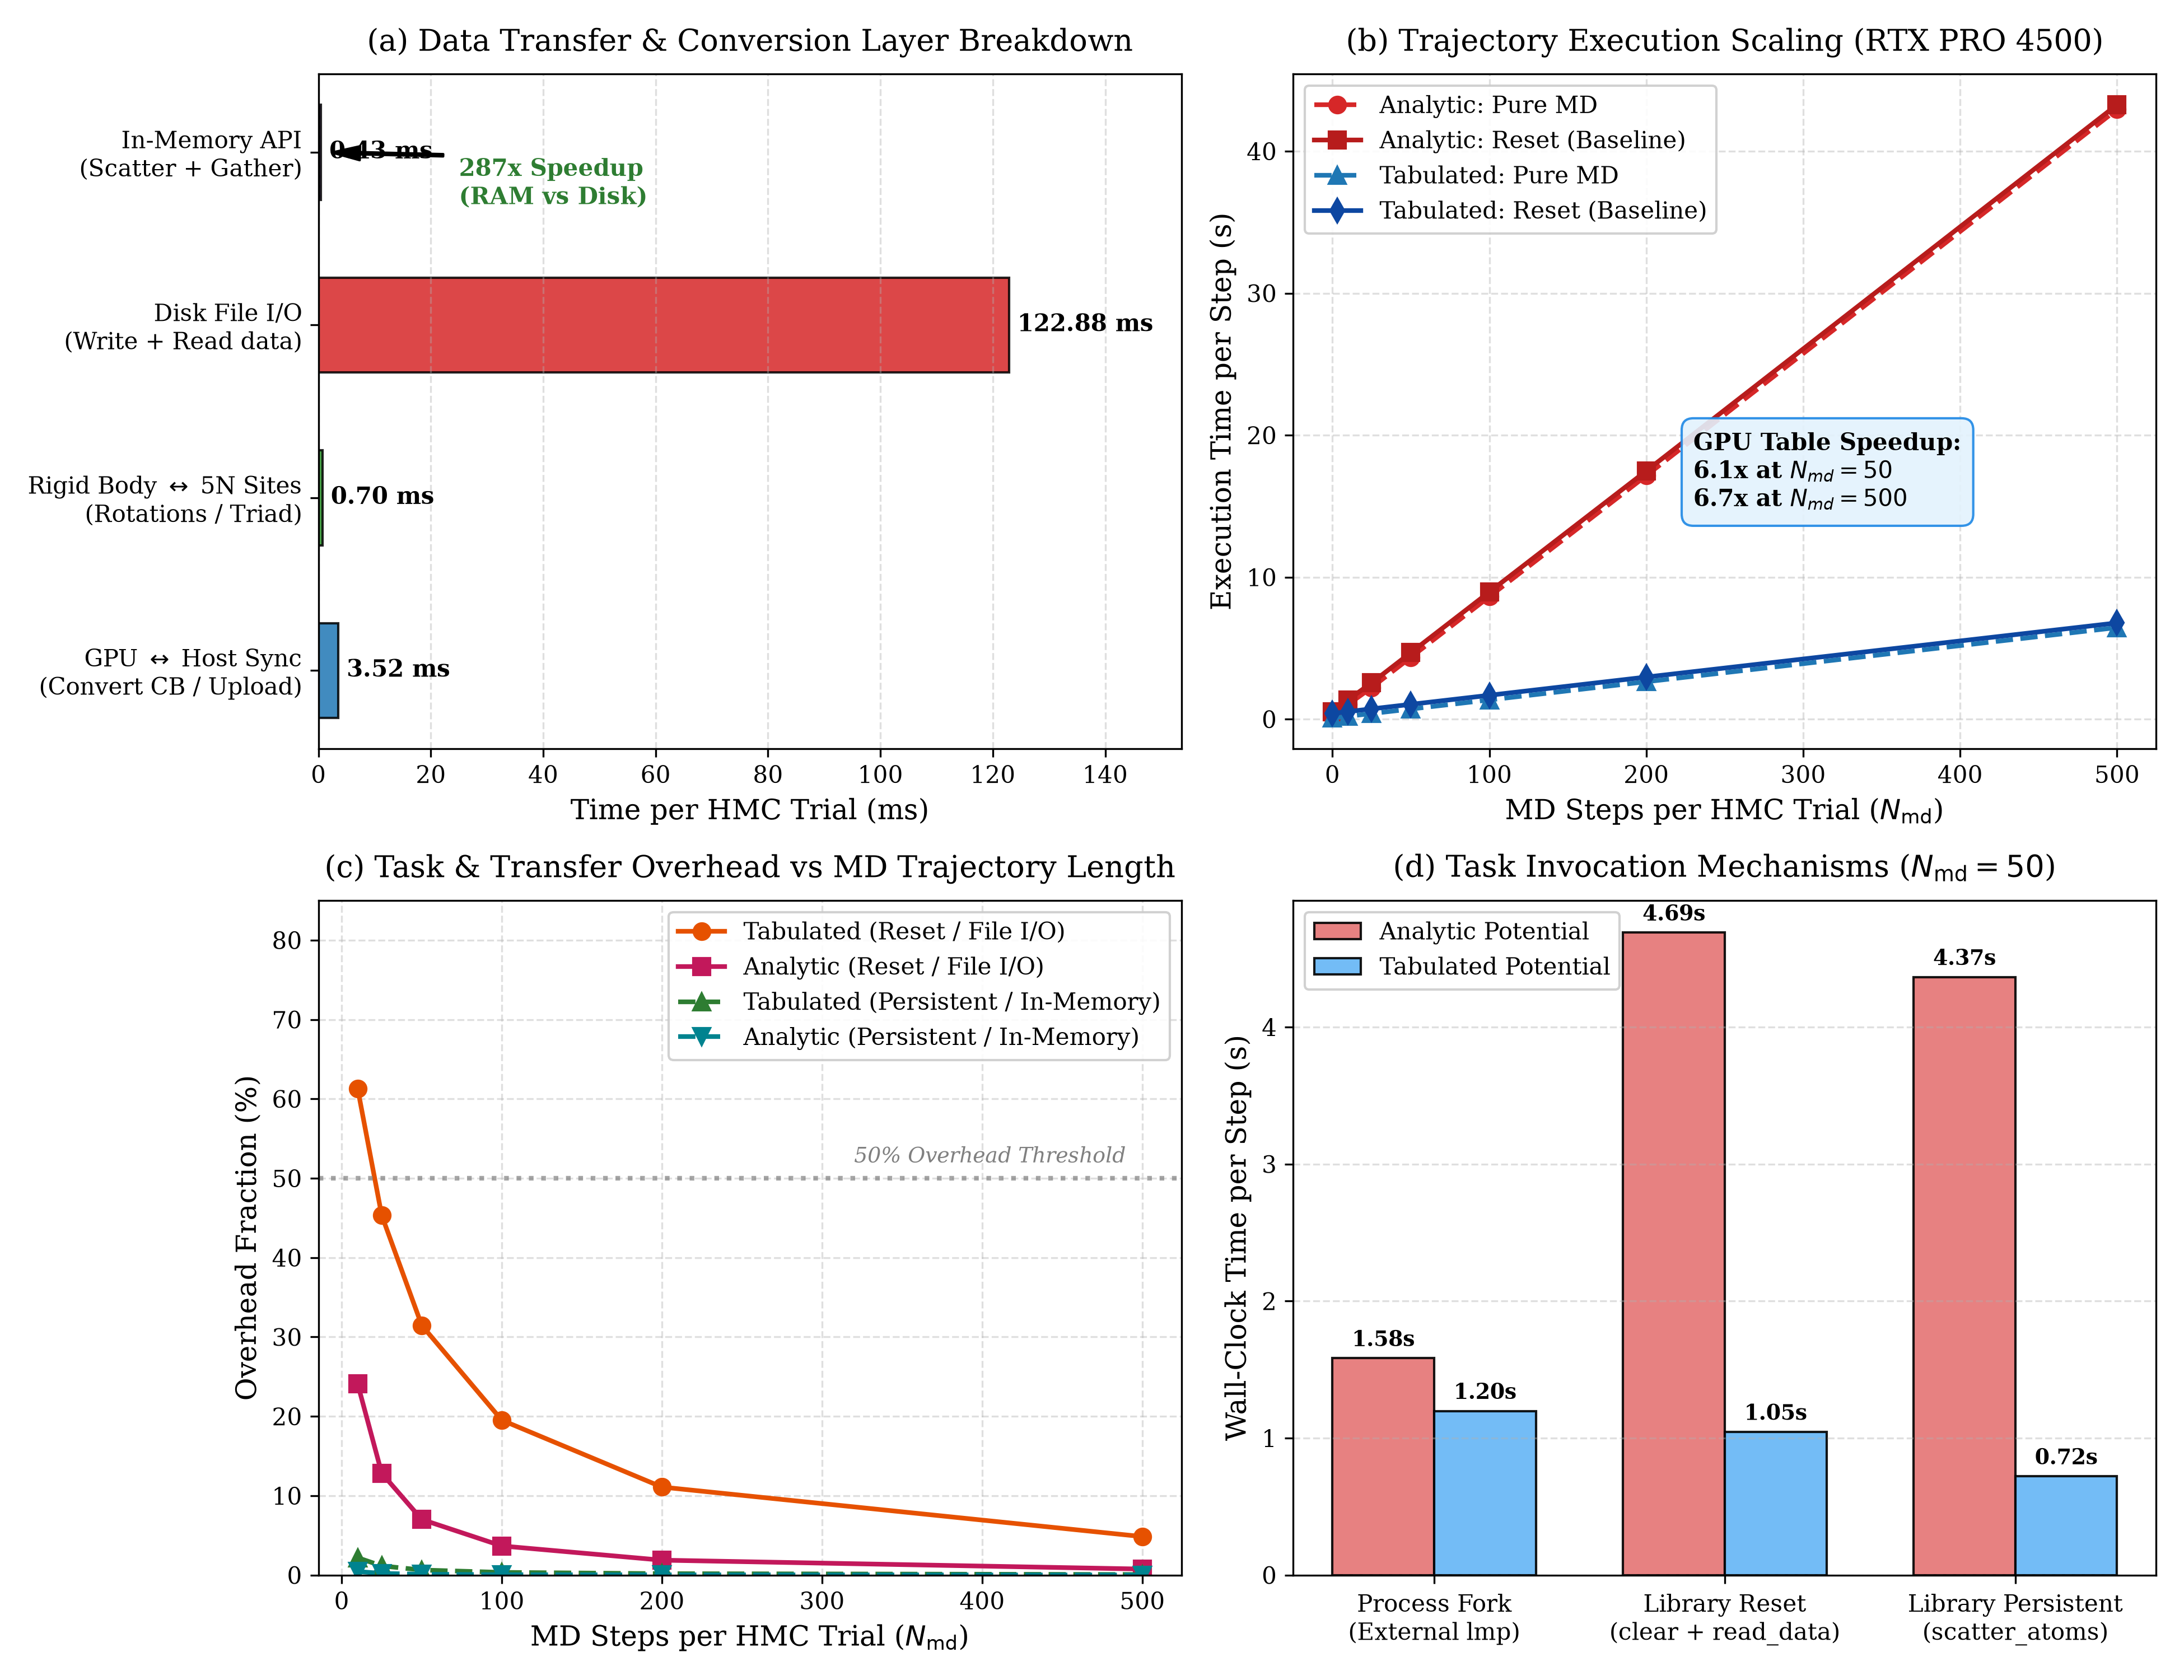
\includegraphics[width=\textwidth]{hmc_overhead_benchmark_comparison.png}
\caption{\textbf{Comprehensive Performance Analysis of Hybrid Monte Carlo (HMC) on NVIDIA RTX PRO 4500}:
(a) Latency breakdown across data transfer and coordinate conversion layers, illustrating the $287\times$ speedup achieved by in-memory API transfer over disk file I/O.
(b) Trajectory execution scaling with respect to MD step count $N_{\mathrm{md}}$, demonstrating a $6.1\times$ to $6.7\times$ throughput advantage for GPU-accelerated tabular potentials over continuous analytic overlays.
(c) Coupling overhead fraction as a function of $N_{\mathrm{md}}$, highlighting the rapid reduction in overhead for persistent in-memory execution ($< 1\%$ for $N_{\mathrm{md}} \ge 25$) versus the baseline reset workflow.
(d) Comparison of task invocation paradigms for $N_{\mathrm{md}} = 50$ steps, contrasting external process forking, in-process library reset (\texttt{clear}), and persistent in-memory execution.}
\label{fig:benchmark_summary}
\end{figure*}

---

\section{Task Invocation and Forking Overhead}

\subsection{The Cost of Re-Initializing Simulation Environments}

In many naive hybrid simulation workflows, external MD software is invoked by either:
\begin{enumerate}
    \item \textbf{External Process Forking}: Spawning an independent operating system process via \texttt{system()} or \texttt{EXECUTE\_COMMAND\_LINE} (e.g., \texttt{mpirun -np 1 lmp -in run.lmp}).
    \item \textbf{In-Process Library Reset}: Maintaining a linked library instance (\texttt{liblammps}) but executing a complete environment teardown via \texttt{clear} at each HMC trial, followed by script parsing and command-line execution.
    \item \textbf{In-Process Persistent State}: Initializing the simulation box, neighbor lists, rigid body fixes, and force fields once, and merely scattering updated coordinates into memory prior to MD propagation.
\end{enumerate}

\begin{table}[b]
\centering
\small
\caption{\textbf{In-Process LAMMPS Task Re-Initialization Overhead} measured across 5 independent trials.}
\label{tab:task_breakdown}
\begin{tabularx}{\textwidth}{lXcc}
\toprule
\textbf{Phase ID} & \textbf{Action / Operation} & \textbf{Time (ms)} & \textbf{Fraction (\%)} \\
\midrule
\texttt{T9}  & LAMMPS \texttt{clear} Command (Memory Deallocation) & $3.874$   & $1.10\%$ \\
\texttt{T4}  & Data File Token Parsing (\texttt{read\_data lammps\_hmc.data}) & $75.010$  & $21.34\%$ \\
\texttt{T10} & Script Parsing \& Fix Definitions (\texttt{pair\_coeff}, \texttt{fix rigid}) & $68.990$  & $19.63\%$ \\
\texttt{T11} & Zero-Step Initialization \& GPU Allocations (\texttt{run 0}) & $203.638$ & $57.93\%$ \\
\midrule
\multicolumn{2}{l}{\textbf{Total Task Re-Initialization Latency ($\Delta T_{\mathrm{task}}$)}} & $\mathbf{351.512}$ & $100.00\%$ \\
\bottomrule
\end{tabularx}
\end{table}

As detailed in Table~\ref{tab:task_breakdown}, issuing \texttt{clear} on every trial incurs a massive overhead of $\mathbf{351.51}$~ms. The largest single contributor is the \texttt{run 0} command ($203.64$~ms), which rebuilds the initial neighbor lists and re-allocates GPU device memory buffers inside the LAMMPS GPU package. Script parsing and fix registration add another $68.99$~ms. When combined with disk file serialization ($47.87$~ms), the total baseline coupling overhead without MD propagation is $\mathbf{403.9}$~ms per HMC trial!

\subsection{External Forking vs. Library Invocations}

Table~\ref{tab:fork_vs_lib} and Figure~\ref{fig:benchmark_summary}(d) compare total wall-clock execution times for a production HMC trial of $N_{\mathrm{md}} = 50$ steps across the three paradigms:
\begin{itemize}
    \item For the \textbf{Tabulated Potential}, persistent in-memory library execution completes the entire HMC step in $\mathbf{0.721}$~s, compared to $1.045$~s for the reset baseline and $1.198$~s for external process forking. Persistent library execution is \textbf{$1.66\times$ faster} than process forking.
    \item For the \textbf{Analytic Potential}, external forking takes $1.583$~s, while library persistent execution takes $4.365$~s. In the analytic case, pure MD integration is significantly slower due to CPU neighbor lists; the external binary's multi-threaded OpenMP scheduling slightly outperforms the single-process library wrapper, but at the expense of process isolation and disk dependencies.
\end{itemize}

\begin{table}[t]
\centering
\small
\caption{\textbf{Task Invocation Paradigm Comparison} for an HMC trial with $N_{\mathrm{md}} = 50$ steps.}
\label{tab:fork_vs_lib}
\begin{tabularx}{\textwidth}{lXccc}
\toprule
\textbf{Interaction Model} & \textbf{Invocation Paradigm} & \textbf{Step Time (s)} & \textbf{Speedup vs. Fork} & \textbf{Overhead (\%)} \\
\midrule
\textbf{Analytic Potential}  & External Process Fork (\texttt{lmp} executable) & $1.583$ & $1.00\times$ & --- \\
(\texttt{neigh no})          & In-Process Library with Reset (\texttt{clear})   & $4.689$ & $0.34\times$ & $7.01\%$ \\
                             & In-Process Library Persistent (\texttt{scatter})& $4.365$ & $0.36\times$ & $\mathbf{0.11\%}$ \\
\midrule
\textbf{Tabulated Potential} & External Process Fork (\texttt{lmp} executable) & $1.198$ & $1.00\times$ & --- \\
(\texttt{neigh yes})         & In-Process Library with Reset (\texttt{clear})   & $1.045$ & $1.15\times$ & $31.47\%$ \\
                             & In-Process Library Persistent (\texttt{scatter})& $\mathbf{0.721}$ & $\mathbf{1.66\times}$ & $\mathbf{0.64\%}$ \\
\bottomrule
\end{tabularx}
\end{table}

---

\section{Trajectory Scaling: Analytic vs. Tabulated Dynamics}

\subsection{Throughput Scaling with Trajectory Length}

Table~\ref{tab:trajectory_scaling} and Figure~\ref{fig:benchmark_summary}(b) document the execution times across trajectory lengths
$N_{\mathrm{md}} \in \{0, 10, 25, 50, 100, 200, 500\}$:
\begin{enumerate}
    \item \textbf{Tabular GPU Acceleration}: In pure MD propagation, tabulated potentials evaluate $N_{\mathrm{md}} = 500$ steps in $\mathbf{6.452}$~s ($12.90$~ms/step), whereas continuous analytic evaluation requires $\mathbf{42.943}$~s ($85.89$~ms/step). The tabulated potential provides a sustained \textbf{$6.66\times$ acceleration} in MD integration.
    \item \textbf{Linear Complexity}: Both potentials scale strictly linearly with $N_{\mathrm{md}}$ ($R^2 > 0.9999$). For tabulated interactions, the marginal computation cost is:
    \begin{equation}
    t_{\mathrm{MD}}^{\mathrm{tab}}(N_{\mathrm{md}}) \approx 0.080 + 0.0127 \times N_{\mathrm{md}} \quad \text{[seconds]}
    \end{equation}
    whereas for analytic interactions:
    \begin{equation}
    t_{\mathrm{MD}}^{\mathrm{ana}}(N_{\mathrm{md}}) \approx 0.196 + 0.0855 \times N_{\mathrm{md}} \quad \text{[seconds]}
    \end{equation}
\end{enumerate}

\begin{table*}[t]
\centering
\small
\caption{\textbf{Trajectory Scaling and Overhead Breakdown} across $N_{\mathrm{md}} \in \{0, \dots, 500\}$ steps. $T_{\mathrm{MD}}$ is pure MD integration time, $T_{\mathrm{base}}$ is baseline execution with environment reset and disk I/O, and $T_{\mathrm{pers}}$ is persistent in-memory execution. $\eta_{\mathrm{base}}$ and $\eta_{\mathrm{pers}}$ are the corresponding overhead percentages.}
\label{tab:trajectory_scaling}
\resizebox{\textwidth}{!}{%
\begin{tabular}{r|cccc|cccc|c}
\toprule
& \multicolumn{4}{c|}{\textbf{Analytic Potential (\texttt{neigh no})}} & \multicolumn{4}{c|}{\textbf{Tabulated Potential (\texttt{neigh yes})}} & \textbf{GPU Table} \\
$N_{\mathrm{md}}$ & $T_{\mathrm{MD}}$ (s) & $T_{\mathrm{base}}$ (s) & $\eta_{\mathrm{base}}$ (\%) & $\eta_{\mathrm{pers}}$ (\%) & $T_{\mathrm{MD}}$ (s) & $T_{\mathrm{base}}$ (s) & $\eta_{\mathrm{base}}$ (\%) & $\eta_{\mathrm{pers}}$ (\%) & \textbf{MD Speedup} \\
\midrule
$0$   & $0.196$  & $0.525$  & $62.63\%$ & $2.31\%$ & $0.080$ & $0.409$ & $80.46\%$ & $5.50\%$ & $\mathbf{2.45\times}$ \\
$10$  & $1.036$  & $1.365$  & $24.09\%$ & $0.45\%$ & $0.208$ & $0.537$ & $61.28\%$ & $2.19\%$ & $\mathbf{4.99\times}$ \\
$25$  & $2.231$  & $2.560$  & $12.84\%$ & $0.21\%$ & $0.397$ & $0.725$ & $45.33\%$ & $1.16\%$ & $\mathbf{5.63\times}$ \\
$50$  & $4.361$  & $4.689$  & $7.01\%$  & $0.11\%$ & $0.716$ & $1.045$ & $31.47\%$ & $0.64\%$ & $\mathbf{6.09\times}$ \\
$100$ & $8.629$  & $8.958$  & $3.67\%$  & $0.05\%$ & $1.355$ & $1.684$ & $19.52\%$ & $0.34\%$ & $\mathbf{6.37\times}$ \\
$200$ & $17.155$ & $17.483$ & $1.88\%$  & $0.03\%$ & $2.638$ & $2.967$ & $11.09\%$ & $0.18\%$ & $\mathbf{6.50\times}$ \\
$500$ & $42.943$ & $43.272$ & $0.76\%$  & $0.01\%$ & $6.452$ & $6.781$ & $4.85\%$  & $0.07\%$ & $\mathbf{6.66\times}$ \\
\bottomrule
\end{tabular}%
}
\end{table*}

\subsection{Crossover Trajectory Length \texorpdfstring{($N_{\mathrm{md}}^*$)}{(N\_md*)}}

The relative overhead of an HMC trial is defined as:
\begin{equation}
\eta = \frac{T_{\mathrm{total}} - T_{\mathrm{MD}}}{T_{\mathrm{total}}} \times 100\%
\end{equation}
As plotted in Figure~\ref{fig:benchmark_summary}(c):
\begin{itemize}
    \item Under \textbf{Baseline Reset}: Because the overhead is dominated by the fixed $\approx 351.5$~ms setup latency, the overhead in the tabulated model remains high for short trajectories ($80.5\%$ at $N_{\mathrm{md}} = 0$, $61.3\%$ at $N_{\mathrm{md}} = 10$). The crossover trajectory length where physical MD represents $\ge 50\%$ of the step time is:
    \begin{equation}
    N_{\mathrm{md}}^* \approx 20 \text{ steps (Tabulated Reset)}
    \end{equation}
    For analytic potentials, because MD integration is slower, the crossover occurs much earlier ($N_{\mathrm{md}}^* \approx 4$ steps).
    \item Under \textbf{Persistent In-Memory Execution}: The total non-MD overhead is reduced to just $4.65$~ms. Consequently, the overhead drops below $\mathbf{1\%}$ for all $N_{\mathrm{md}} \ge 25$ steps ($\eta = 0.64\%$ at $N_{\mathrm{md}} = 50$, and $0.07\%$ at $N_{\mathrm{md}} = 500$). This virtually eliminates any coupling bottleneck, allowing users to select $N_{\mathrm{md}}$ purely based on physical sampling efficiency and acceptance probability.
\end{itemize}

---

\section{Conclusions and Best Practices}

We have performed a rigorous, microsecond-resolved profiling investigation of the Hybrid Monte Carlo (HMC) integration in \texttt{MC\_Checkerboard} for a cluster-forming system of $N = 7{,}695$ tetrahedral patchy colloids ($38{,}475$ interaction sites). Our findings establish clear architectural principles for hybrid MC/MD codes:
\begin{enumerate}
    \item \textbf{Eliminate Disk File Transfers}: Disk file serialization and parsing consumes over $120$~ms per trial ($96.7\%$ of transfer latency). In-memory pointer communication via \texttt{scatter\_atoms} and \texttt{gather\_atoms} achieves a \textbf{$287\times$ acceleration}, reducing coordinate exchange latency to $0.43$~ms.
    \item \textbf{Maintain Persistent In-Memory State}: Re-initializing the simulation environment via \texttt{clear} wastes $351.5$~ms per trial in neighbor-list rebuilds and GPU context allocation. Operating with persistent topology fixes reduces total coupling overhead to $4.65$~ms ($< 1\%$ overhead for $N_{\mathrm{md}} \ge 25$).
    \item \textbf{Leverage GPU-Accelerated Tabulated Potentials}: Hardware-interpolated linear tables with GPU-native neighbor lists accelerate pure MD integration by up to \textbf{$6.66\times$} compared to continuous analytic overlays on the GPU.
    \item \textbf{Optimal Trajectory Regimes}: For production HMC simulations using tabulated potentials, choosing $N_{\mathrm{md}} \in [50, 200]$ ensures that physical MD integration represents $> 99\%$ of the compute time while maintaining near-unity Metropolis acceptance rates ($P_{\mathrm{acc}} \approx 100\%$).
\end{enumerate}

These implementations and benchmark test cases are permanently archived in the \texttt{MC\_Checkerboard} repository under \nolinkurl{test_cases/hmc_lammps_overhead_benchmark/}, providing fully reproducible artifacts for the computational molecular simulation community.

\section*{Acknowledgments}
Computational resources and support provided by the Scientific Computing Center of CSIC (\textit{Supercomputaci\'{o}n CSIC}, Ladon cluster) and financing through the Spanish Ministry of Science, Innovation and Universities.

\begin{thebibliography}{99}
\bibitem{sciortino2007patchy}
F.~Sciortino, \textit{Eur. Phys. J. B} \textbf{2007}, \textit{64}, 505--509.

\bibitem{palaia2022patchy}
I.~Palaia, et al., \textit{ACS Nano} \textbf{2022}, \textit{16}, 3918--3928.

\bibitem{bianchi2006phase}
E.~Bianchi, J.~Largo, P.~Tartaglia, E.~Zaccarelli, F.~Sciortino, \textit{Phys. Rev. Lett.} \textbf{2006}, \textit{97}, 168301.

\bibitem{rovigatti2018simulate}
L.~Rovigatti, J.~Russo, F.~Romano, \textit{Eur. Phys. J. E} \textbf{2018}, \textit{41}, 67.

\bibitem{whitelam2007avoiding}
S.~Whitelam, P.~L. Geissler, \textit{J. Chem. Phys.} \textbf{2007}, \textit{127}, 154101.

\bibitem{duane1987hybrid}
S.~Duane, A.~D. Kennedy, B.~J. Pendleton, D.~Roweth, \textit{Phys. Lett. B} \textbf{1987}, \textit{195}, 216--222.

\bibitem{mehlig1992hybrid}
B.~Mehlig, D.~W. Heermann, B.~M. Forrest, \textit{Phys. Rev. B} \textbf{1992}, \textit{45}, 679.

\bibitem{forrest1990hybrid}
B.~M. Forrest, U.~W. Suter, \textit{Mol. Phys.} \textbf{1990}, \textit{70}, 847--857.

\bibitem{miller2002symplectic}
T.~F. Miller, M.~Eleftheriou, P.~Pattnaik, A.~Ndirango, G.~J. Martyna, \textit{J. Chem. Phys.} \textbf{2002}, \textit{116}, 8649--8659.

\bibitem{neal2011mcmc}
R.~M. Neal, \textit{Handbook of Markov Chain Monte Carlo} \textbf{2011}, \textit{2}, 113--162.

\bibitem{gonzalez2026checkerboard}
E.~G. Noya, A.~D\'{i}az-Pozuelo, E.~Lomba, \textit{J. Chem. Theory Comput.} \textbf{2026}, submitted.

\bibitem{thompson2022lammps}
A.~P. Thompson, et al., \textit{Comp. Phys. Comm.} \textbf{2022}, \textit{271}, 108171.
\end{thebibliography}

\end{document}
